% Generated by scripts/build_latex.py -- do not edit by hand.
% Regenerate with:  python scripts/build_latex.py
\documentclass[preprint,12pt,number]{elsarticle}

\usepackage[T1]{fontenc}
\usepackage{lmodern}
\usepackage{textcomp}
\usepackage{amsmath}
\usepackage{amssymb}
\usepackage{graphicx}
\usepackage{booktabs}
\usepackage{siunitx}
\usepackage{rotating}
\usepackage{adjustbox}
\usepackage[hidelinks]{hyperref}
\usepackage{url}

\graphicspath{{figures/}}
\sisetup{detect-all}
\biboptions{numbers,sort&compress}

% Pandoc emits these for tightlist and passthrough spans.
\providecommand{\tightlist}{\setlength{\itemsep}{0pt}\setlength{\parskip}{0pt}}
\providecommand{\passthrough}[1]{#1}

\journal{Chemometrics and Intelligent Laboratory Systems}

\begin{document}

\begin{frontmatter}

\title{The Exactly-Determined Reference Panel: Why Two-Sample Slope-and-Bias Recalibration Cannot Be Checked, and Why Larger Panels Are Not Reliably Safe Either}

%% Author block withheld for double-anonymised review; supplied in the
%% separate title-page file.
\author{}
\address{}

\begin{abstract}
Slope-and-bias correction is the cheapest way to keep a multivariate calibration usable after an instrument has drifted, and the practical question is how many freshly referenced samples it needs. We evaluate it on a five-channel metal-oxide gas-sensor array against co-located reference-analyser values over 389 days, freezing the held-out set of each 30-day target window before any reference is selected. Three analytes, three model classes and ten target windows give 90 decision cells at each of ten reference budgets from 0 to 50, and the evaluation is repeated under ten independent reference-panel draws. Replication proves essential: one draw yields an apparently clean threshold at four references, which does not reproduce, instead ranging from 4 to 20. We therefore report only draw-invariant results. First, the exactly-determined panel is a distinct regime, because a two-parameter correction fitted on two samples has no residual degrees of freedom and so cannot be contradicted by the data that produced it; correspondingly, calibration-slope inversion and inflation beyond fivefold occur at two references and at no other budget in any draw, the worst case inflating normalised RMSE 44.5-fold against 4.7-fold anywhere above two. Second, the failure is genuinely tail-shaped: that inversion arises in one draw of ten, while the median sequence at two references is near-neutral in every draw. Third, no small panel is reliably safe, failures above twice frozen error persisting to ten references and clearing in every draw only at twenty. A pre-decision diagnostic predicts how much error will be recovered (Spearman 0.581--0.852 on 121 previously unused days, in all ten draws) but does not order sequences by safety at two references. The operational rule is therefore a prohibition on exactly-determined panels with inspection of panel geometry, not a sample-size threshold.
\end{abstract}

\begin{keyword}
calibration transfer; model updating; slope and bias correction; standardization set size; gas sensor array; instrumental drift; tail risk
\end{keyword}

\end{frontmatter}
\subsection{1. Introduction}

\subsubsection{1.1 Model updating is the routine response to instrumental drift}

A multivariate calibration built on one instrument, at one time, in one
environment, rarely stays valid. In gas-sensing the response of a metal-oxide
array to a fixed concentration changes with sensor aging, temperature and
humidity, operating history, and the composition of the sample matrix, so the
mapping from response to concentration degrades over the deployment period
{[}1,2{]}. Field studies of low-cost air-quality devices report that a calibration
obtained in the laboratory does not transfer to deployment, and that the drift
has to be assessed over the intended operating interval rather than assumed
away {[}3{]}. The same problem in near-infrared spectroscopy motivated the
calibration-transfer literature, where the response of a secondary instrument is
standardized to a primary one, or the model is updated, using a small set of
samples measured on both {[}4,5{]}.

Two vocabularies describe one activity. Calibration transfer usually treats a
spatial problem, moving a model between instruments; drift compensation usually
treats a temporal one, moving a model between times on the same instrument. The
algebra of the cheapest remedy is identical in both. If the drifted predictions
retain their ordering and only their scale and offset have moved, a two-parameter
correction of the model output restores them, and this is the method that
calibration transfer knows as slope-and-bias or bias-and-skew correction {[}5,6{]}.
It is the least invasive option available, it needs no access to the original
training data, and it is the option a working laboratory reaches for first.

\subsubsection{1.2 The unresolved question is the size of the reference set}

Every update method needs freshly referenced samples, and those samples are the
dominant cost. In a gas-sensing deployment each one requires a co-located
reference analyser reading; in process spectroscopy each requires a wet-chemistry
assay. The operational question is therefore not which correction is most
accurate in principle but \textbf{how few referenced samples the correction can be
trusted with}.

The calibration-transfer literature is unusually explicit that this number is
small, and unusually vague about how small. Piecewise direct standardization was
introduced with a handful of transfer samples {[}4{]}; reviews describe slope-and-bias
correction as requiring only a modest set and note that the requirement depends
on how the samples span the range {[}5,6{]}; subsequent work emphasises the selection
of representative transfer samples precisely because the count is low enough for
individual samples to matter {[}7{]}. In gas sensing, reviews of calibration update
for electronic noses identify reference-sample availability as the binding
practical constraint {[}1{]}. Yet reported guidance is typically an average
performance at one or two set sizes, or a percentage of the target data, rather
than a curve over an absolute count with the failure modes attached
{[}8--11{]}.

An average is the wrong summary for a decision about a minimum. A laboratory
choosing a reference budget is not trying to optimise expected error; it is
trying to avoid a corrected instrument that reads backwards. Those are different
objectives and, as we show, they are answered by different statistics.

\subsubsection{1.3 What a small reference set actually does}

The cost of an undersized reference set does not appear in the centre of the
distribution. At two references the typical sequence is unaffected, with a median
ratio of corrected to frozen error between 0.964 and 1.094 across ten independent
panel draws. Yet in one of those draws three sequences invert the calibration slope,
turning the corrected instrument into one that reports high concentrations as low,
the worst inflating error 44.5-fold. The other nine show no inversion at all.

That combination --- a neutral centre, a rare and unbounded failure --- is a tail risk,
and it has an uncomfortable methodological consequence. Whether a deployment meets
the failure depends on which samples it happens to draw, so a single evaluation
cannot tell a laboratory what its risk is. Our own first analysis used one draw and
found an apparently clean threshold: nothing above twice frozen error from four
references onward. Nine further draws gave thresholds spanning 4 to 20. Four is the
modal value, so the original analysis was not unlucky, merely uninformative about a
spread reaching twenty.

We therefore organise the paper around what replicates and what does not, and the
part that replicates is structural. A two-parameter correction fitted on two samples
interpolates both, so its residual is identically zero and \textbf{no statistic computed
from the panel can reveal that it has failed}; its coefficient is a ratio of
differences whose denominator is small precisely when the model has lost resolution
and can change sign precisely when the model has degraded most (Section 2.1).
Consistent with this, inversion and inflation beyond fivefold occur at two references
and at no other budget, in any draw. At three a residual degree of freedom appears
and unbounded failure disappears --- which does not make three safe: moderate failures
persist to ten references in some draws. The regime boundary is at exact
determination, and there is no second boundary that makes a small panel trustworthy.

\subsubsection{1.4 Contributions}

\begin{enumerate}
\def\labelenumi{\arabic{enumi}.}
\tightlist
\item
  \textbf{A regime distinction rather than a threshold}, separating the
  exactly-determined panel from all larger ones on structural grounds and confirming
  it across 900 decision cells per budget.
\item
  \textbf{A demonstration that the sample-size threshold does not replicate}, with
  per-draw values from 4 to 20, reported as a negative result about single-draw
  evaluation of standardization-set size because our own first analysis produced the
  clean answer and it was wrong.
\item
  \textbf{Mechanism, with the panel geometry made explicit}: the exact arithmetic by which
  a range-spanning two-sample panel inverts.
\item
  \textbf{A pre-decision diagnostic with its scope honestly bounded}, including a search
  for a panel-side guard that would have licensed two-sample correction and the two
  respects in which it fails.
\item
  \textbf{Threshold and endpoint sensitivity as part of the result}, reporting the grid
  over criterion and error metric rather than one cell of it.
\end{enumerate}

This paper does not propose a new correction algorithm, a new drift-compensation
model, or a new transfer-sample selection method. It does not attribute the
observed temporal change to a specific physical drift mechanism, and it does not
construct a traceable uncertainty budget for the reference values. Its
contribution is a regime boundary with a mechanism, and an explicit account of what
this class of evaluation can and cannot establish.

\subsection{2. Background and problem formulation}

\subsubsection{2.1 Slope-and-bias correction as the minimal update}

Let a calibration \(f\) be fitted on source data and let \(\mathbf{x}\) denote the
sensor response in a later target period. Output correction replaces \(f\) by

\[\tilde{f}(\mathbf{x}) = a + b\,f(\mathbf{x}),\]

with \(a\) and \(b\) estimated by least squares on a panel of \(N\) target-period
samples for which reference values are available. The correction assumes the
drifted model preserves the ordering of concentrations and has moved only in
scale and offset. Nothing in the feature space is altered and the source data are
not revisited, which is why the method is standard practice when the drift is
mild and the reference budget is tight {[}5,6{]}.

Two properties of this estimator drive everything that follows. First, it needs
at least two distinct reference values, and with exactly two it is determined:
for a panel of two samples with reference values \(y_1 < y_2\) and drifted
predictions \(\hat y_1, \hat y_2\),

\[b = \frac{y_2 - y_1}{\hat y_2 - \hat y_1}.\]

The estimate is therefore a ratio of two differences, and it is unbounded as the
denominator approaches zero and changes sign with it. Second, the fitted line
interpolates both points exactly, so the residual vector is zero regardless of
whether \(b\) is sensible. The estimator is simultaneously most fragile and least
checkable at \(N = 2\).

At \(N \ge 3\) the least-squares solution is no longer a single pairwise ratio and
the panel acquires \(N - 2\) residual degrees of freedom, so a badly conditioned
panel can in principle announce itself. We return to whether it does so in
practice in Section 4.5.

\subsubsection{2.2 How many standardization samples does the literature recommend?}

Calibration transfer treats the size of the standardization set as small and
sample-selection-sensitive rather than as a quantity with a published minimum.
Piecewise direct standardization was demonstrated with a small number of transfer
samples spanning the calibration range {[}4{]}; the review literature describes
slope-and-bias correction as the oldest and simplest transfer method and stresses
that its adequacy depends on how well the chosen samples cover the range
{[}5,6{]}. Work on transfer-sample selection is motivated explicitly by the
observation that when the count is this low, \emph{which} samples are chosen alters the
result {[}7{]}. The recurring recommendation is that the samples span the
concentration range, which is the design we adopt and which, as Section 4.4
shows, is also what makes the two-sample case dangerous.

In gas sensing the corresponding literature is largely algorithmic: feature-space
correction {[}12,13{]}, ensemble adaptation over batches {[}8,9,14{]}, domain adaptation and
distribution alignment {[}15,16{]}, semi-supervised and online exploitation of unlabelled
target data {[}17,18,19{]}, and calibrant-free approaches that avoid references altogether
{[}20{]}. These target accuracy under drift and generally report a single panel design or a
fraction of target data, so the complementary question --- the smallest trustworthy
reference count for the cheapest correction --- is not usually the object of study, and
reported averages cannot answer it. Adaptive network calibration of air-quality devices
is closer to our setting {[}21{]}, and the corpus we use originates in on-field calibration
of exactly this kind {[}22,23{]}.

\subsubsection{2.3 Estimand, endpoints, and the tail statistic}

The decision unit is a \textbf{cell}: an (analyte, target window, model class) triple.
A laboratory deploys one model for one analyte and decides on an action for it, so
the action is chosen per cell. The reporting unit for association analyses is the
temporal sequence (analyte, target window), with per-model results given
separately.

For each cell and each budget \(N\) we compute normalised RMSE on the frozen
held-out set,

\[\mathrm{nRMSE} = \frac{\mathrm{RMSE}}{\max(y) - \min(y)},\]

for the frozen model and for the corrected model, and form the per-cell ratio

\[r = \frac{\mathrm{nRMSE}_{\text{corrected}}}{\mathrm{nRMSE}_{\text{frozen}}}.\]

We report the mean and median of \(r\) and, as failure endpoints, the \textbf{count of cells
with \(r\) above a threshold} and the \textbf{worst \(r\) observed}. A threshold of two is a
coarse statement of unacceptability --- a corrected instrument with twice the error of
the uncorrected one is a failed intervention, not a marginal outcome --- but it is not a
privileged value, and Section 4.2 shows the budget at which the count vanishes depends
on it. We therefore report counts at 1.5, 2, 3 and 5 times frozen error, on MAE as
well as normalised RMSE. The worst observed ratio is reported alongside because it is
what a prohibition actually bounds and needs no threshold, as does the count of cells
whose held-out calibration slope is negative, which isolates the inversion subclass.

Because both strategies in a ratio are scored on the same held-out set, the range
normaliser of nRMSE is identical in numerator and denominator and cancels: \(r\) is
exactly the ratio of raw RMSEs. Conclusions drawn from \(r\) therefore do not depend
on the choice of normaliser, although the absolute nRMSE values do.

The held-out calibration slope is the slope of a regression of reference values on
predictions computed on the test set, where unity is ideal. It is a different
quantity from the correction coefficient \(b\) of Section 2.1, and the two differ by
an order of magnitude in the failure cases; we keep them notationally distinct
throughout.

Two summaries are avoided. Recovery ratios of the form

\[\frac{\mathrm{nRMSE}_{\text{frozen}} - \mathrm{nRMSE}_{\text{corrected}}}
{\mathrm{nRMSE}_{\text{frozen}} - \mathrm{nRMSE}_{\text{oracle}}}\]

are unstable when the denominator is small and are reported only as secondary
quantities with denominator diagnostics. Cells are not treated as independent
replicates: they share source fits and target windows, so dispersion is descriptive
and no pooled confidence statement is made across them.

\subsubsection{2.4 A diagnostic available before the decision}

A quantity that is to inform the decision must be computable without the held-out
set. Let \(\mathrm{nRMSE}_{\text{frozen}}(\text{panel})\) be the frozen model scored
on the \(N\) reference samples and \(\mathrm{nRMSE}_{\text{source val}}\) the same
model family scored on the latest source window withheld from its own training.
Define

\[D_{\mathrm{ref}}(N) = \frac{\mathrm{nRMSE}_{\text{frozen}}(\text{panel}) -
\mathrm{nRMSE}_{\text{source val}}}{\mathrm{nRMSE}_{\text{source val}}},\]

the relative degradation of the deployed model on the reference panel compared
with its own source-period performance. Both terms are available at the moment of
the decision. This distinguishes \(D_{\mathrm{ref}}\) from test-set degradation
measures, which are observable only after the fact and therefore cannot drive an
operational rule --- a limitation of the analysis this manuscript supersedes.

The pre-specified hypotheses were: \(D_{\mathrm{ref}}(5)\) is positively associated
with the absolute benefit of correction (H1); a rule that corrects only when
\(D_{\mathrm{ref}}(N) \ge \tau\) beats both always-frozen and always-correct on
held-out mean nRMSE (H2); and the reference count needed for the \emph{action} to
stabilise is smaller than the count needed for the \emph{fit} to plateau (H3).
Section 3.6 records the provenance of these hypotheses, which is not neutral and
is disclosed as part of the result.

\subsection{3. Materials and methods}

\subsubsection{3.1 Corpus}

The evidence corpus is the De Vito air-quality array, a five-channel metal-oxide
gas-sensor device co-located with certified reference analysers at an urban
roadside site over 389 days from 10 March 2004 to 4 April 2005, distributed
through the UCI Machine Learning Repository {[}24{]} and originating in on-field
calibration studies of the same device {[}22,23{]}.

Three analytes are used, each with a co-located reference-analyser target: CO in
mg m$^{-3}$, NO$_2$ in \si{\micro\gram\per\cubic\metre}, and NOx in ppb. Features are the five metal-oxide channels
PT08.S1(CO), PT08.S2(NMHC), PT08.S3(NOx), PT08.S4(NO$_2$) and PT08.S5(O$_3$). The
sentinel value $-$200 is treated as missing and complete cases are formed per
analyte over the target and the five channels. The NMHC reference channel is
excluded because 8443 of 9357 rows are sentinel. Temperature, relative humidity
and absolute humidity are excluded as features so that the temporal signal is not
absorbed by contemporaneous environmental covariates.

Two properties make this corpus suitable for a claim about reference-set size,
and they are the properties the withdrawn version of this work lacked. Target
values are reference-analyser readings rather than supplied nominal levels, and
each 30-day window contains between 40 and 478 distinct reference values per
analyte (Table~\ref{tab:table1}). A reference set spanning a genuine working range is a
precondition for any statement about how many samples that range needs.

A second corpus is retained for contrast only. The W\"orner one-year electronic-nose
archive {[}25{]} carries two nominal concentration levels per analyte and 6--12
held-out rows per sequence. It cannot support a statement about a concentration
range and is used solely for the comparison in Section 4.7.

\subsubsection{3.2 Temporal windows and leakage control}

Windows are 30 days wide, counted from the first timestamp, giving 13 windows over
the 389-day span. Windows 1--3 are the source period and each of windows 4--13 is
evaluated as a target period in turn, giving 10 target windows and, with three
analytes, \textbf{30 temporal sequences} and \textbf{90 decision cells} at each budget.

Within each target window, 30 \% of rows are assigned to a held-out test set,
stratified into ten quantile bins of the reference value, \textbf{before any reference
sample is selected}. A concentration stratum containing a single row is left in
the reference pool because it cannot be represented in both the calibration and
the evaluation set. The test set is then fixed for all budgets and all strategies,
so every comparison in this paper is made against an identical held-out set.
Temporal order is validated programmatically and no random split across time is used,
following the standard cautions on cross-validation under temporal dependence {[}26,27,28{]}
and on target leakage {[}29{]}. This is not a generic precaution in this corpus family: an
audit of a widely used metal-oxide benchmark found recording batches temporally clustered,
with residual drift sufficient to identify the batch, so random splits overstated
performance {[}30{]}. A random split here would let a target window's later hours inform the
fit for its earlier ones --- precisely the information a deployment lacks.

Analysis is additionally restricted to the concentration range common to the
source period and the target window, so that no strategy is credited or penalised
for extrapolating outside the range the source model was built on.

\subsubsection{3.3 Reference panels}

Reference budgets are absolute counts, \(N \in \{0, 2, 3, 4, 5, 6, 8, 10, 20,
50\}\), and panels are \textbf{nested}: the panel at a larger budget contains the panel
at every smaller one, so budget effects are not confounded with panel identity.

Panels are ordered to span the reference range, as calibration-transfer practice
recommends {[}5,7{]}. Concretely, the reference pool of each sequence is sorted by
quantile stratum and drawn in the order lowest, highest, second lowest, second
highest, and so on. The first two samples are therefore one row from the lowest
stratum and one from the highest. This maximises the leverage available to a
two-point fit, which is the intended behaviour, and it is also the mechanism behind
the failures reported in Section 4.4.

Within a stratum the specific row is selected by a pseudo-random permutation under
a fixed seed, so a panel is one realisation of a family of admissible
range-spanning panels. \textbf{The entire evaluation is repeated under ten seeds}
(20260826, the protocol's seed, and 11, 22, 33, 44, 55, 66, 77, 88, 99), each of
which redraws every panel and reseeds the model random states. This gives ten
independent replicates of the whole design, 900 decision cells per budget in total,
and it is the basis for separating draw-invariant results from draw-specific ones
throughout Section 4.

The replication was added after the primary analysis, as a post-hoc robustness
check. It changes no threshold, hypothesis, or verdict of the frozen protocol; it
tests whether the protocol's descriptive findings survive a nuisance parameter.
The primary draw retains its status as the pre-specified analysis and is identified
as such wherever per-draw results are given.

\subsubsection{3.4 Models and update strategies}

Three model classes are used: PLS regression with two components on standardized
features, a random forest with 200 trees, and gradient-boosted trees with 300
rounds, depth 5 and learning rate 0.05. Hyperparameters are fixed in advance and
are not tuned per window, because tuning per target window would itself consume
target-period information.

Four strategies receive the identical reference panel:

\begin{itemize}
\tightlist
\item
  \textbf{frozen} --- the source model, unchanged. The reference panel is not used.
\item
  \textbf{output correction} --- the source model with the two-parameter correction of
  Section 2.1 fitted on the panel. This is the lightweight strategy under study.
\item
  \textbf{target-only refit} --- a new model of the same class fitted on the panel alone,
  discarding the source data.
\item
  \textbf{full retraining} --- a new model of the same class fitted on the source data
  and the panel together.
\end{itemize}

At \(N = 0\) the correction is undefined and every strategy degenerates to the
frozen model, which is why the \(N = 0\) row of every table reports a ratio of
exactly one. This row is retained because it fixes the reference level of the
comparison.

\subsubsection{3.5 Endpoints}

The primary endpoint is held-out nRMSE and the primary decision statistic is the
count of cells with ratio above two, as specified in Section 2.3. Secondary
endpoints are MAE, the held-out calibration slope, and a recovery ratio reported
with denominator diagnostics. The reported association tests are Spearman rank
correlations, chosen because the relation between \(D_{\mathrm{ref}}\) and recovered
error is not assumed linear and because the ratio scale is heavy-tailed.

\subsubsection{3.6 Pre-specification, provenance, and a disclosed confound}

The protocol was frozen in writing before the benchmark was executed
(\texttt{docs/uci360\_primary\_protocol.md}), and no threshold, window boundary, or verdict
was altered afterwards. Two features of its provenance are disclosed because they
bear on how the results should be weighted.

\textbf{The diagnostic hypothesis is exploratory in origin.} \(D_{\mathrm{ref}}\) and the
form of the decision rule were devised by inspecting an earlier three-window
analysis of this same corpus covering its first 270 days. Target windows 4--9
overlap that span and are therefore \textbf{in-sample for hypothesis generation};
windows 10--13, covering 5 December 2004 to 4 April 2005, are 121 days that no
earlier analysis in this project examined and constitute the confirmation set.
Results are reported separately for the two sets throughout, and the held-out set
carries the evidential weight. The hypothesis is not presented as pre-registered
from the outset of the project.

\textbf{The diagnostic and the correction share a panel.} \(D_{\mathrm{ref}}(N)\) is
computed on the same \(N\) samples used to fit the correction. Selecting a large \(N\)
therefore improves the quality of the fit for reasons unrelated to the quality of
the decision, so the choice of decision budget in H2 does not isolate the
diagnostic's value. Comparisons between the rule and the always-correct baseline
at a fixed \(N\) remain valid and are the ones we interpret.

Additionally, the mechanism analysis of Section 4.5 and Table~\ref{tab:tables3} is \textbf{post-hoc}.
It was constructed after the failures were observed, is not among H1--H3, and is
reported as mechanism and as a negative result rather than as a validated rule.

\subsubsection{3.7 Reproducibility}

The benchmark was executed twice from the same configuration and seed in
independent output directories. Row keys are identical, both runs produce
2160 $\times$ 22 tables on the pre-specified grid, and the maximum absolute numerical
difference across all numeric columns is 2.487 $\times$ 10$^{-1}$$^3$, consistent with
floating-point accumulation alone. Missing-value patterns are identical in every
numeric column and all three pre-specified verdicts, both decision budgets, and
the held-out association coefficient reproduce exactly. Figures are regenerated
from the result tables by script and reproduce byte-identically on re-execution.

\subsection{4. Results}

Results are reported at two levels. The \textbf{primary draw} is the pre-specified
analysis under the protocol's seed, 90 decision cells per budget with no skipped
sequences, and it is the basis of Tables 1--4. The \textbf{replicated analysis} pools
ten draws, 900 cells per budget, and is used wherever a claim about reference count
is at issue. Where the two disagree we say so and the replicated result
governs.

\subsubsection{4.1 The mean and the median disagree, but only when the tail is realised}

Fig.~\ref{fig:1} shows held-out error against reference count for the primary draw, with
mean and median plotted on the same axes. They agree everywhere except at the
smallest budget. At two references the median ratio is \textbf{1.009}, the typical
sequence being neither helped nor harmed, while the mean ratio is \textbf{2.005}.
Removing the eight cells above twice frozen error takes the remaining 82 from a
mean frozen error of 0.191 to a corrected 0.161, a ratio of \textbf{0.845}: once the
tail is excluded, two references are already beneficial on average.

The divergence is itself draw-dependent, which is the correct behaviour for a
tail-driven mean rather than a defect. Across the ten draws the median at two
references stays within 0.964--1.094 while the mean spans 0.979--1.149 in the nine
non-inverting draws against 2.005 in the primary one. The mean departs from the median
exactly in the draw whose tail materialised, so a mean reported from a single
evaluation carries an unstated dependence on whether that evaluation was unlucky.

Two statements about central tendency survive all ten draws: the median at two
references is within 10 \% of unity in every draw, and it falls below one at four
references in every draw (0.885--0.984) but not at three (0.934--1.025). Median benefit
therefore begins at four references, consistently. In the primary draw absolute error
decreases monotonically in both mean and median from four references through to fifty,
where the mean ratio is 0.729 and 83 of 90 cells improve; the median \emph{ratio} is not
monotone, rising slightly at six and twenty, and we claim no monotone ratio
improvement.

\subsubsection{4.2 The failure threshold does not replicate}

Fig.~\ref{fig:2} shows every cell at every budget for the primary draw together with the
count exceeding twice frozen error. In that draw the count is \textbf{8 at two
references, 4 at three, and zero at four and above} --- an apparently clean
threshold at four.

It does not replicate. Under nine further panel draws the budget from which a draw
and all larger budgets are clean takes the values 4, 4, 4, 4, 4, 5, 6, 8, 20 and 20
(Table~\ref{tab:table5}, and Fig.~\ref{fig:5}b). Four is modal, so the pre-specified draw was typical rather
than unlucky --- which is the point: a typical draw still gives no information about
the spread, and the spread reaches twenty. Pooled over all 900 cells per budget the
twofold criterion is first met by every draw at \textbf{twenty} references. The statement
``no sequence exceeds twice its frozen error from four references onward'' is a
property of a panel realisation and we retract it.

The apparent threshold is sensitive to the criterion as well, independently of the
draw (Table~\ref{tab:tables5}). In the primary draw the first clean budget is 4 at a twofold
criterion, 3 at threefold and fivefold, and 50 at 1.5-fold, because two cells remain
above 1.5 at twenty references. Measuring error by MAE rather than normalised RMSE
moves it from 4 to 8, one NOx sequence sitting just above twice frozen MAE at four,
five and six references while falling just below on nRMSE. A threshold statement is
thus a joint function of the draw, the criterion and the metric, none of which is
canonical. What survives is a bound, reported next.

\subsubsection{4.3 Unbounded failure occurs at two references and nowhere else}

The endpoint that does replicate is the worst case, which requires no threshold.
Table~\ref{tab:table6} gives it pooled over ten draws and 900 cells per budget, and two features are
draw-invariant.

\textbf{Slope inversion occurs at two references and at no other budget in any draw}, and
the same holds for inflation beyond fivefold. Above two references the worst outcome
anywhere in 900 cells per budget is 4.7-fold and decays with panel size; at two it is
44.5-fold, an order of magnitude larger, and unbounded in principle for the reason
given in Section 2.1. Both catastrophic events occur in \textbf{one of the ten draws} ---
the substance of calling this a tail risk, since nine laboratories in ten would have
seen a worst case between 2.25 and 4.62 and concluded the exactly-determined panel
merely mediocre.

Beyond exact determination the decay is gradual and offers no second boundary. Cells
above twice frozen error fall 48, 25, 10, 8, 5, 3, 3 and reach zero only at twenty
references; cells above threefold persist to eight. There is no small panel size at
which residual risk becomes negligible.

\subsubsection{4.4 Where the correction goes wrong}

Fig.~\ref{fig:3} shows the held-out calibration slope by budget for the primary draw. At
zero references, that is for the uncorrected frozen model, the median slope is
1.175: the deployed models overpredict the concentration range and this is the
distortion the correction is asked to remove. From two references onward the median
slope approaches unity monotonically, from 0.786 at two to 0.988 at fifty.

Three cells at two references have a negative slope, minimum $-$0.120, meaning the
corrected model orders concentrations backwards. No inversion occurs at any larger budget
in this draw --- the minimum at three references is +0.354 --- nor above two in any draw.

Dispersion behaves differently from the median, and the intuitive reading is wrong. The
standard deviation of the slope is 0.240 at two references, \textbf{smaller} than the 0.331 at
three, because two-point fits are displaced downward as a group rather than scattered. It
contracts decisively only at the largest budgets, 0.126 at twenty and 0.088 at fifty. The
distribution therefore tightens on unity late, and these data would not support a claim
that precision improves steadily with reference count.

\subsubsection{4.5 Mechanism: a two-point fit inverts when the panel is compressed}

Because panels are ordered to span the range, the two-reference panel consists of
one sample from the lowest quantile stratum and one from the highest. In the NO$_2$
window that carries all three inversions those samples have reference values of
\textbf{27.0 and 118.0 \si{\micro\gram\per\cubic\metre}}, a true gap of +91.0.

All three frozen models place them in the wrong order (Table~\ref{tab:tables2}). PLS predicts
116.60 and 112.33, the random forest 117.32 and 107.66, and the gradient-boosted
model 122.64 and 110.94, giving predicted gaps of \textbf{$-$4.27, $-$9.66 and $-$11.70}. By
the two-point identity of Section 2.1 the correction coefficients are therefore
\textbf{$-$21.32, $-$9.42 and $-$7.78}, and every prediction is inverted. Held-out error
inflates 44.5-, 23.8- and 19.8-fold.

Both causes of the magnitude matter. The sign of the denominator produces the inversion;
its smallness produces the size, since a 91 \si{\micro\gram\per\cubic\metre} interval compressed into four units of
predicted range yields a coefficient of twenty before the sign is considered. A correction
that looks like a modest two-parameter adjustment is in fact a division by a quantity the
laboratory has not inspected.

That window is the sparsest of the ten NO$_2$ windows (362 rows, 106 distinct reference
values), the lowest in mean concentration at 66.0 \si{\micro\gram\per\cubic\metre}, and the most strongly
right-skewed at 0.60 (Table~\ref{tab:tables4}); its range is not the narrowest, so the distinguishing
features are sparsity and low concentration rather than range. This is the regime in which
a drifted model has least resolution to order two samples correctly.

\subsubsection{4.6 Two references cannot be checked, and three can only be checked weakly}

The two-parameter correction fitted on two points reproduces both exactly. The
median residual RMSE over the reference panel at two references is \textbf{0.000} and
the residual degrees of freedom are zero (Table~\ref{tab:tables3}). No statistic computed from
the reference panel can distinguish the three inverting cells from the rest on
goodness-of-fit grounds, because all of them fit perfectly.

We searched for a panel-side guard that would permit two references with a
safeguard instead of forbidding them, and report that it does not hold.

The sign of the predicted gap over the panel does separate the inversion subclass
perfectly: the three cells with a non-positive predicted gap are exactly the three
largest inflations, and no other cell at two references has one. This costs nothing and
is available before the decision, so we recommend it as a screen. It does not license
the exactly-determined panel, for two reasons. First, the remaining \textbf{five of eight}
failures at two references have \emph{positive} predicted gaps --- compression without
inversion, which the sign test cannot see. Second, at three references, where a residual
degree of freedom exists, the four surviving failures look \textbf{clean on their own panel}:
rank agreement between predicted and reference ordering is 1.000 in every case and the
panel correlation exceeds 0.98, with only a mildly elevated residual (median 13.4
against 4.05). Each of those panels has two closely spaced low references and one
distant high reference, so the fit is determined by a single leveraged point and
reproduced almost exactly.

The operational consequence is that no panel-side statistic licenses the
exactly-determined case, and that the check which does work there --- the sign of the
predicted gap --- is a prohibition condition rather than a gate that can be traded
against sample size. At two references the correction cannot be checked at all; at
three it can be checked, and the check passes on cells that fail.

\subsubsection{4.7 The diagnostic predicts recovery but does not confer safety}

Fig.~\ref{fig:4} shows \(D_{\mathrm{ref}}\) against realised benefit at five references and at
two, with rule-fitting and held-out windows distinguished.

At five references the diagnostic is strongly associated with the magnitude of the
benefit on the confirmation windows: in the primary draw Spearman \(\rho = 0.814\),
\(p = 1.6 \times 10^{-9}\), \(n = 36\), against \(\rho = 0.348\) on the rule-fitting windows,
which are in-sample for hypothesis generation (Table~\ref{tab:table4}). This is the one substantive
result that replicates without qualification --- across the ten draws the held-out
coefficient ranges from 0.581 to 0.852, all \(p < 0.001\) --- so the diagnostic's
predictive content is a property of the method, not of a panel realisation.

Its safety content is not. At two references the association weakens and loses
consistency across window sets in the primary draw (\(\rho = 0.372\) held-out,
\(\rho = -0.120\) rule-fitting, \(\rho = 0.201\) pooled, \(p = 0.057\)). In that draw the
three cells with the \textbf{highest} diagnostic values are the three catastrophic ones,
with \(D_{\mathrm{ref}}\) between 5.15 and 5.94, and the top diagnostic quartile has a
mean ratio of 4.43 against a median of 0.665 --- whereas at five references that same
quartile has the \emph{best} mean ratio, 0.568.

That reversal is draw-specific and we do not generalise it: in the nine draws without
an inversion the top diagnostic quartile at two references has mean ratios between
0.541 and 0.991, no worse than the rest and usually better. The defensible statement
is weaker and still sufficient. At two references the diagnostic does not order
sequences by safety, and the primary draw is an existence proof that its highest
values can coincide with total failure, so a gate keyed on a high diagnostic can
recommend correction precisely where the exactly-determined fit is about to fail even
though it will not usually do so. The diagnostic answers ``how much will this recover?''
and not ``is this safe to attempt?''

H2, the rule-utility hypothesis, is technically supported and practically null
(Table~\ref{tab:table4}). The rule beats always-correct by 0.041 \% on the confirmation windows while
correcting 35 of 36 sequences: it is always-correct plus rounding. The honest reading,
which the frozen protocol anticipated and declared reportable, is that \textbf{above exact
determination no gate is needed}, because almost every sequence benefits. H3 is
supported --- action agreement with the largest-budget diagnostic reaches 100 \% at ten
references while the fit does not plateau until twenty --- so deciding whether to
correct is cheaper than correcting well.

\subsubsection{4.8 The prohibition belongs to the correction, not to the deployment}

Table~\ref{tab:table2} compares all four strategies on identical panels. Target-only refitting, which
discards the source model, is markedly worse at small budgets: in the primary draw its
mean nRMSE is 0.456 at two references against 0.296 for output correction, worst ratio
40.5, and \textbf{35 of 90 cells} above twice frozen error against eight.

The ordering replicates exactly where the threshold did not. \textbf{In all ten draws,
target-only refitting has a higher mean nRMSE than output correction at every budget
from two to twenty, and a lower one only at fifty} --- the crossing point is identical
in every draw. Within this strategy the mean misleads in the same way it did for
output correction: target-only mean nRMSE falls below the frozen model's at four
references (0.178 against 0.184), so a mean-based reading would license four, while
its mean per-cell ratio does not fall below one until eight.

Full retraining behaves in the opposite way from both. It never exceeds twice frozen
error at any budget in any draw, because the source data dominate the fit and bound
the damage a bad panel can do, but it improves slowly, from 0.173 at two references to
0.123 at fifty, and is the least effective of the three update strategies from five
references onward. If a laboratory must act on an exactly-determined panel and cannot
refuse, full retraining is the only option we tested that cannot invert.

Retaining the source model and correcting only its output is thus what makes a
small panel usable at all, and the comparison fixes the scope of everything above.
The prohibition on exactly-determined panels is a statement about output
correction; the strategies differ in how badly they fail and in whether they can
fail without bound, so minimum-reference guidance is a property of the update
method rather than of the instrument or the deployment.

\subsubsection{4.9 The regime boundary is only observable on a corpus with a working range}

Applying the identical protocol to the two-level contrast corpus {[}25{]} at five
references gives 12 sequences improved against 12 worsened. The same protocol on
this corpus gives 59 against 31.

The difference is a property of the reference structure, and it bounds where a claim
about reference-set size can be made at all. With two nominal concentration levels there
is no range over which a slope can be estimated: the correction of Section 2.1
degenerates towards an offset adjustment, because \(b\) comes from a single contrast that
every panel reproduces identically. Reference \emph{count} then has almost no room to act, and
such a corpus will show heterogeneity across analytes and models rather than a dependence
on count --- not because the dependence is absent but because the design cannot express it.
Studies evaluating calibration update against nominal levels, common where reference
analysers are unavailable, are therefore structurally unable to detect a reference-count
effect. The regime distinction reported here required 40 to 478 distinct values per window
(Table~\ref{tab:table1}).

\subsection{5. Discussion}

\subsubsection{5.1 Principal interpretation}

Two conclusions of different kinds come out of this evaluation, and separating them is
the point.

The first is structural and firm. The exactly-determined reference panel is a distinct
regime, not the small end of a continuum: its coefficient is a ratio of differences
that can be arbitrarily small or negatively signed, and its residual is identically
zero, so nothing in the panel can reveal that this has happened. Across 900 decision
cells per budget and ten panel draws, inversion and inflation beyond fivefold occur at
two references and nowhere else. We regard this as the durable result, because the
reasoning is a property of the estimator and the empirical pattern is what that
reasoning predicts.

The second is a negative result about how such questions are usually answered. Asking
where the safe boundary lies is the natural next step, and it has no stable answer
here. Our first analysis, on one draw, found nothing above twice frozen error from four
references onward; nine further draws spread that boundary over 4 to 20, a threefold
criterion moves it to three, a 1.5-fold criterion removes it up to fifty, and measuring
on MAE moves it to eight. The boundary is a joint function of draw, criterion and
metric, and reporting any single combination as \emph{the} minimum reference count would be
a mistake we nearly made.

What replaces it is a bound and a prohibition. Above exact determination the worst
outcome anywhere is 4.7-fold and decays with panel size, with no point at which
residual risk becomes negligible --- failures above twice frozen error persist to ten
references in some draws. A laboratory cannot buy safety with a slightly larger panel;
it can only avoid the regime where failure is unbounded, then inspect what it drew.
This is less convenient than a minimum sample size, and it may explain why the
literature's guidance on standardization-set size is expressed as loosely as it is
{[}5,6,7{]}: the quantity being sought may not be stable enough to state as a number.

\subsubsection{5.2 Why two samples is a special case rather than a small case}

The structural argument of Sections 2.1 and 4.5 is the part of this work we expect
to generalise most directly, because it is a property of the estimator rather than
of the corpus.

A two-parameter correction on two points is exactly determined. Its coefficient is a
ratio of differences whose denominator is the drifted model's predicted gap over the
panel --- small precisely when the model has lost resolution, and able to invert precisely
when the model has degraded most --- while the fit interpolates both points, so its
residual carries no information. The estimator is least stable and least checkable at the
same sample size. Any method estimating \(k\) parameters from \(k\) referenced samples
inherits this, so the argument extends to bias-only correction at one sample and to
higher-order corrections at their own exact-determination point.

This also explains why spanning the range, which calibration transfer correctly
recommends {[}5,7{]}, is not protective there. Spanning maximises the denominator in
expectation and is the right design, but it cannot prevent that denominator from being
small or negative in the particular window where the model has drifted worst. Good
transfer-sample design and an adequate transfer-sample count are separate requirements.
The draw sensitivity of Section 4.2 is the same point from another angle: every one of our
ten draws is a valid range-spanning panel chosen by the recommended design, yet they
differ by a factor of twenty in worst case at two references. Design fixes the family of
panels a laboratory might draw, not which one it gets.

\subsubsection{5.3 Relation to the calibration-transfer and drift-compensation literature}

Our result is consistent with the standing description of slope-and-bias
correction as effective with a modest reference set {[}5,6{]}, and it puts a number and
a failure mode on ``modest'' for this class of instrument. It is also consistent with
the emphasis in transfer-sample selection work on the sensitivity of the outcome to
which samples are chosen {[}7{]}: at the counts where that sensitivity is largest, we
find it is not merely a matter of efficiency but of whether the correction inverts.

Relative to the gas-sensor drift-compensation literature, this paper is
deliberately not an algorithmic contribution. Feature-space methods such as
component correction and orthogonal signal correction {[}12,13{]}, ensemble adaptation
{[}8,9,14{]}, distribution alignment {[}15,16{]}, and semi-supervised or online updating
{[}17,18,19{]} pursue accuracy under drift and often assume a supply of target-period
data. Calibrant-free approaches {[}20{]} avoid the reference requirement entirely and
are the appropriate choice when no references can be obtained. Our contribution is
orthogonal: for the cheapest and most widely used correction, it establishes the
count below which the correction should be refused, and the reason.

The corpus originates in on-field calibration of a co-located array {[}22,23{]} and
subsequent work on the same platform has addressed adaptive network calibration
over time {[}21{]}. That line of work supports the premise that periodic output
correction is a realistic operational practice; the present result specifies its
minimum input.

\subsubsection{5.4 Recommended procedure}

Every step uses only quantities available before the correction is committed.

\begin{enumerate}
\def\labelenumi{\arabic{enumi}.}
\tightlist
\item
  \textbf{Never fit an output correction on an exactly-determined panel}, meaning never on
  two samples for the two-parameter form. This is a prohibition resting on the
  estimator's structure, not a threshold to trade against sampling cost. With only two
  references, leave the model frozen or use full retraining, which bounded the damage
  at every budget in every draw.
\item
  \textbf{Inspect the panel before fitting, at every count.} Check that the drifted model
  orders the reference samples as the reference method does and that their spread is a
  substantial fraction of the reference spread; a non-positive or negligible predicted
  spread is a refusal condition. This detects inversion but not compression or
  single-point leverage (Section 4.6), so it is necessary and not sufficient.
\item
  \textbf{Do not treat a modest panel as safe because it clears a published minimum.}
  Failures above twice frozen error persisted to ten references in some draws and
  cleared everywhere only at twenty, so prefer the largest panel the budget allows
  rather than the smallest meeting a criterion.
\item
  \textbf{Above exact determination, correct without a gate.} A diagnostic-gated rule beat
  unconditional correction by 0.041 \%, not worth the complexity. Use
  \(D_{\mathrm{ref}}\) to anticipate how much will be recovered, not to decide whether
  to proceed.
\item
  \textbf{Budget the decision separately from the fit}, since the action stabilises near ten
  references while the fit improves to about twenty.
\item
  \textbf{Do not substitute a target-only refit at small budgets}: worse than output
  correction at every budget below fifty in every draw.
\end{enumerate}

\subsubsection{5.5 What it costs to evaluate a tail rather than a mean}

Two design requirements follow from studying a rare failure, and both are more
demanding than the conventional reporting of an average at a given set size.

\textbf{Enough sequences for the event to appear.} A failure occurring in 8 of 90 cells is
as likely as not to be absent entirely from a design with eight sequences, and an
evaluation that missed it would have reported two references as neutral --- exactly what
the mean says. Corpus scale here is not statistical power in the usual sense but a
precondition for observing the endpoint at all.

\textbf{Enough panel draws for the estimate to mean anything.} This is the requirement we
underestimated. One draw produced a clean, plausible, wrong answer, and nothing internal
to that analysis signalled the problem: reproducibility passed to 2.5 $\times$ 10$^{-1}$$^3$, the tail
count decayed monotonically, and the mechanism matched the observed failures. Only
redrawing exposed it. Any study reporting a minimum standardization-set size from a
single sample selection is exposed to the same error, and we would now regard
replication over draws as mandatory rather than as a robustness appendix. Ten draws is
itself few --- the per-draw boundary ranges over 4 to 20 --- so we report a bound rather
than an estimate.

\subsection{6. Limitations}

\textbf{One instrument and one site.} All results come from a single five-channel array
at one urban roadside location. The structural argument of Section 5.2 should
transfer because it concerns the estimator; every empirical quantity here should be
re-established elsewhere before being relied on.

\textbf{Ten draws demonstrate instability without characterising it, and the catastrophic
case rests on few events.} Per-draw boundaries span 4 to 20 with a mode of 4, enough
to show that the threshold is unstable and that the pre-specified draw was typical, but
not to describe the boundary's distribution. The frequency with which a two-sample
panel inverts --- one draw in ten, a single event --- is an observation, not an estimate.
The positive occurrence rests on three cells, all in that draw and all three model
classes of one NO$_2$ window, the sparsest and lowest in concentration of the ten;
confinement of inversion to exact determination holds across all 900 cells per budget,
but the supporting event count is three.

\textbf{Cells are not independent, and threshold dependence is reported rather than
resolved.} The 90 cells per draw share source fits and target windows and the 900
pooled cells share the corpus, so dispersion statistics are descriptive and the
draw-to-draw comparison is one of realisations, not a sampling distribution. Likewise
we show that the apparent boundary depends on criterion and error metric without
offering a principled choice among them; a laboratory with a defined tolerance should
read the relevant column of Table~\ref{tab:tables5} rather than adopt ours.

\textbf{Parts of the analysis are exploratory in origin, as disclosed in Section 3.6.} The
diagnostic hypothesis was generated on windows overlapping the rule-fitting set, so the
confirmation windows carry the evidential weight for H1, and the shared panel means the
H2 decision budget does not isolate the diagnostic's contribution. The mechanism
analysis of Section 4.6 and Table~\ref{tab:tables3} was built after the failures were observed and is
reported as mechanism and as a negative result on a candidate guard, not as a validated
screening rule.

\textbf{Temporal change is not attributed to physical drift, and predictive error is not
measurement uncertainty.} We describe a change in the joint distribution of sensor
response and reference value between windows without separating sensor aging from
environmental variation, maintenance, or concentration-distribution shifts;
environmental covariates were excluded as features, which prevents the temporal signal
being absorbed but also means we cannot apportion it. nRMSE and the held-out
calibration slope are predictive statistics, not statements of trueness or of
measurement uncertainty in the metrological sense, and no traceability claim is made
beyond what the source corpus documents.

\textbf{Three model classes.} Other families, in particular neural approaches with different
extrapolation behaviour, may compress a reference range differently and would change how
often the exactly-determined panel fails.

\subsection{7. Conclusions}

For slope-and-bias recalibration of a drifting metal-oxide gas-sensor array against
co-located reference-analyser values, the exactly-determined reference panel is a
distinct regime rather than the small end of a continuum. A two-parameter correction
fitted on two samples has no residual degrees of freedom, so it cannot be contradicted
by the data that produced it, and its coefficient is a ratio of differences whose
denominator is small precisely when the drifted model has lost resolution and can
change sign precisely when it has degraded most. Across ten panel draws and 900
decision cells per budget, inversion and inflation beyond fivefold occur at two
references and at no other budget, the worst case inflating normalised RMSE 44.5-fold
through a correction coefficient of $-$21.3, against 4.7-fold anywhere above two.

The failure is genuinely tail-shaped, which carries a methodological consequence we
report as a result in its own right. That inversion appears in one draw of ten while
the median sequence at two references is near-neutral in every draw, so a single
evaluation cannot establish a safe reference count: our first analysis found nothing
above twice frozen error from four references onward, and nine further draws spread
that boundary over 4 to 20, with further movement under a different criterion or error
metric. We retract the threshold and report a bound instead. No small panel is reliably
safe --- failures above twice frozen error persist to ten references and clear in every
draw only at twenty.

The operational rule is consequently a prohibition with an inspection, not a sample
size. Never fit an output correction on an exactly-determined panel; check in every
case that the drifted model orders the reference samples correctly and spreads them
appreciably, which detects inversion though not compression; and expect residual risk
across the whole range of panel sizes a laboratory would consider. A pre-decision
diagnostic predicts how much error will be recovered, with held-out Spearman
coefficients of 0.581 to 0.852 in all ten draws, but does not order sequences by safety
at two references. Target-only refitting was worse than output correction at every
budget below fifty in every draw, so guidance of this kind belongs to a specific update
method rather than to an instrument or a deployment.

\subsection{Declarations}

\subsubsection{Data availability}

The corpus is the public De Vito air-quality dataset, available from the UCI
Machine Learning Repository under DOI 10.24432/C59K5F and cited as {[}24{]}. The
contrast corpus is available from Zenodo under DOI 10.5281/zenodo.15681119 and
cited as {[}25{]}. A reproducibility package containing the protocol document,
analysis scripts, configuration files, schema audit, complete benchmark tables,
run manifests, and figure- and table-generation scripts is supplied as
supplementary material. A DOI-bearing archival record will be created before
submission and reported to the editor through non-review metadata.

\subsubsection{Code availability}

All code, configurations, the frozen protocol, the complete benchmark tables, and
the figure and table generation scripts are supplied as supplementary material.
Every number in Sections 4 and 5 and in Tables 1--4 and S1--S4 is produced by
\texttt{generate\_uci360\_tables.py} and \texttt{generate\_uci360\_figures.py} from the archived
result files, and both scripts record their own SHA-256 in the artefacts they
write.

\subsubsection{Ethics statement}

This study reanalyses public archives of non-human sensor measurements and does not
involve human participants, animals, or identifiable personal data. No
institutional ethics approval was required.

\subsubsection{Funding}

Provided in the separate title-page file.

\subsubsection{Declaration of competing interests}

Provided as a separate submission file.

\subsubsection{Author contributions (CRediT)}

Provided in the separate title-page file.

\subsubsection{Declaration of generative AI and AI-assisted technologies}

During the preparation of this work the author used AI-assisted tools to support
bibliographic organisation, code and documentation review, drafting and editing,
and formatting. After using these tools the author reviewed and edited the content
as needed and takes full responsibility for the content of the published article.


\clearpage

%% ---- Figures ----

\begin{figure}[htbp]
\centering
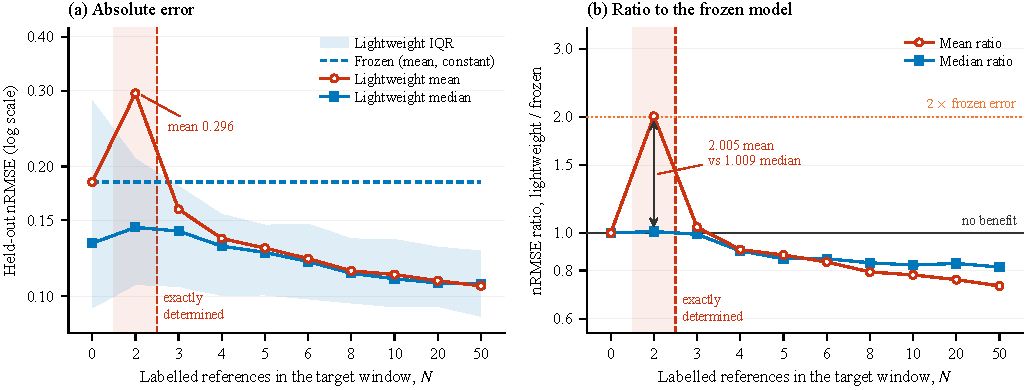
\includegraphics[width=\textwidth]{figure_01_budget_curves.pdf}
\caption{Held-out nRMSE of lightweight output recalibration against the number of labelled target-window references $N$, pooled over 90 decision cells (3 analytes $\times$ 3 model classes $\times$ 10 target windows). (a) Absolute error, with the frozen source model shown for reference and the interquartile range of the recalibrated model shaded. (b) The same result as a ratio to the frozen model, with a double arrow marking the mean--median gap at $N=2$. Mean and median are plotted together because they disagree at the smallest budget: at $N=2$ the median cell is essentially unaffected (ratio 1.009) while the mean is inflated to 2.005 by a small number of cells. From $N=4$ both statistics fall below 1 together (0.906 mean, 0.899 median), and absolute error then falls monotonically in both mean and median across the remaining budgets. The mean--median divergence at $N=2$ is specific to draws in which the tail is realised: across the ten draws of Figure 5 the median at $N=2$ is 0.964--1.094, whereas the mean is 2.005 here and 0.979--1.149 in the other nine. Vertical axes are logarithmic in both panels; budgets are drawn at equal spacing, not to numeric scale, so that the small-panel region remains legible. Lower is better.}
\label{fig:1}
\end{figure}

\begin{figure}[htbp]
\centering
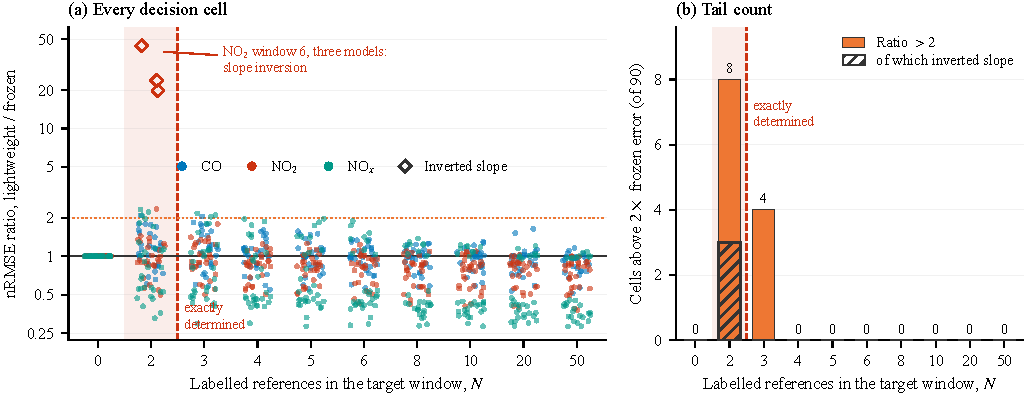
\includegraphics[width=\textwidth]{figure_02_tail_decay.pdf}
\caption{(a) Ratio of recalibrated to frozen held-out nRMSE for every decision cell at each budget (90 cells per budget), coloured by analyte and jittered horizontally; open diamonds mark cells whose fitted calibration slope is negative. The bulk of the distribution lies near or below 1 at every budget, including $N=2$. (b) Number of cells exceeding twice the frozen error: 8 at $N=2$, 4 at $N=3$, and none from $N=4$ onward; the hatched overlay counts the subset with an inverted slope (3 cells, all at $N=2$). The three largest inflations are the three model classes of the same NO$_2$ window.}
\label{fig:2}
\end{figure}

\begin{figure}[htbp]
\centering
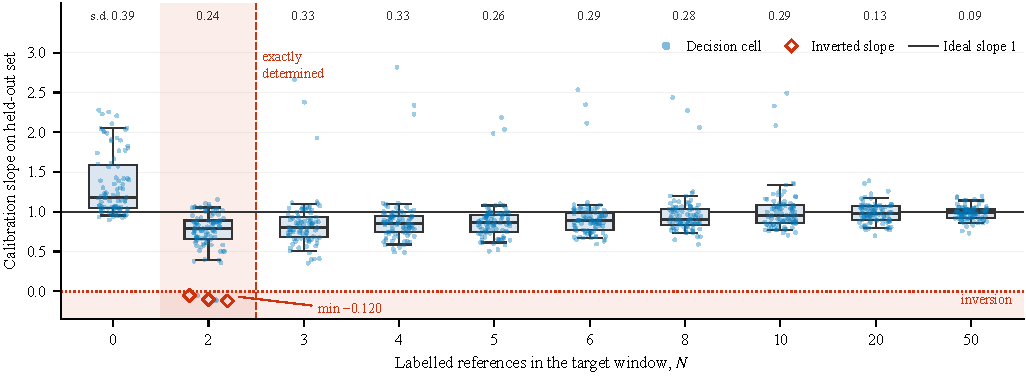
\includegraphics[width=\textwidth]{figure_03_slope_convergence.pdf}
\caption{Distribution of the calibration slope against reference budget, where the plotted quantity is the slope of a regression of reference-analyser values on model predictions over the held-out test set and 1 is ideal. It is not the calibrator's own fitted coefficient. Boxes show the interquartile range and median with 5th--95th percentile whiskers; individual decision cells are overlaid. $N=0$ is the frozen model's held-out slope, that is, the distortion the calibrator is asked to remove (median 1.175). A two-point fit at $N=2$ can invert the slope entirely (minimum $-0.120$, 3 cells in the shaded inversion band), which reverses every prediction. No inversion occurs at any larger budget (minimum 0.354 at $N=3$). The median slope then approaches unity monotonically, from 0.786 at $N=2$ to 0.988 at $N=50$. Dispersion behaves differently and is printed above each box: the standard deviation is 0.240 at $N=2$, which is \emph{smaller} than the 0.331 at $N=3$, because two-point fits are displaced downward as a group rather than scattered. Dispersion contracts decisively only at the largest budgets (0.126 at $N=20$ and 0.088 at $N=50$). Budgets are drawn at equal spacing, not to numeric scale.}
\label{fig:3}
\end{figure}

\begin{figure}[htbp]
\centering
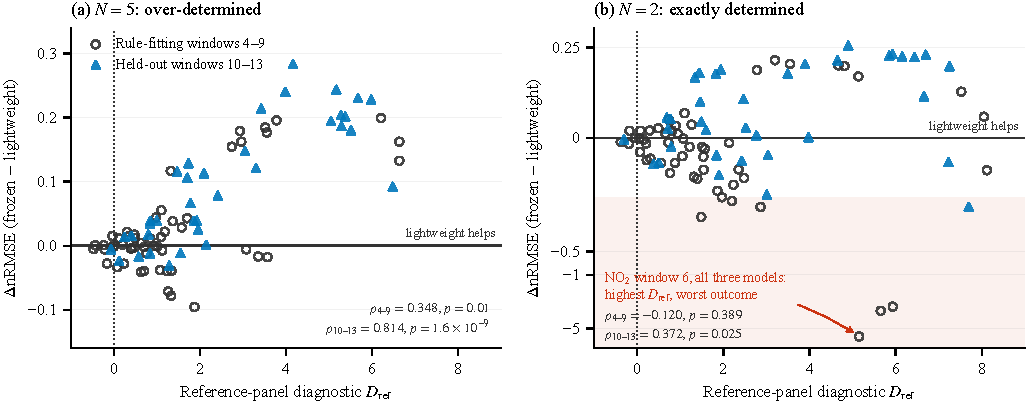
\includegraphics[width=\textwidth]{figure_04_diagnostic.pdf}
\caption{Reference-panel diagnostic $D_{\mathrm{ref}}$, computed before any recalibration decision, against the realised benefit $\Delta$nRMSE $=$ nRMSE$_{\mathrm{frozen}}-$nRMSE$_{\mathrm{lightweight}}$. Open circles are the rule-fitting windows 4--9, filled triangles the held-out windows 10--13. (a) At $N=5$ the diagnostic predicts the magnitude of the gain (Spearman $\rho=0.814$, $p=1.6\times 10^{-9}$ on held-out windows; $\rho=0.348$, $p=0.01$ on rule-fitting windows). (b) At $N=2$ the association is much weaker and no longer consistent across window sets ($\rho=0.372$, $p=0.025$ held-out; $\rho=-0.120$, $p=0.389$ rule-fitting; $\rho=0.201$, $p=0.057$ pooled). More important than the weakening is the direction of the failures: the three cells with the highest diagnostic values are the three catastrophic ones, so the association that survives at $N=2$ does not order cells by safety. Note the symmetric logarithmic vertical axis in (b), linear within $\pm0.1$, and the different vertical ranges of the two panels. A gate keyed on a high diagnostic therefore recommends recalibration exactly where a two-point fit is about to fail, which is why the prohibition has to be a hard constraint rather than something the diagnostic can manage.}
\label{fig:4}
\end{figure}

\begin{figure}[htbp]
\centering
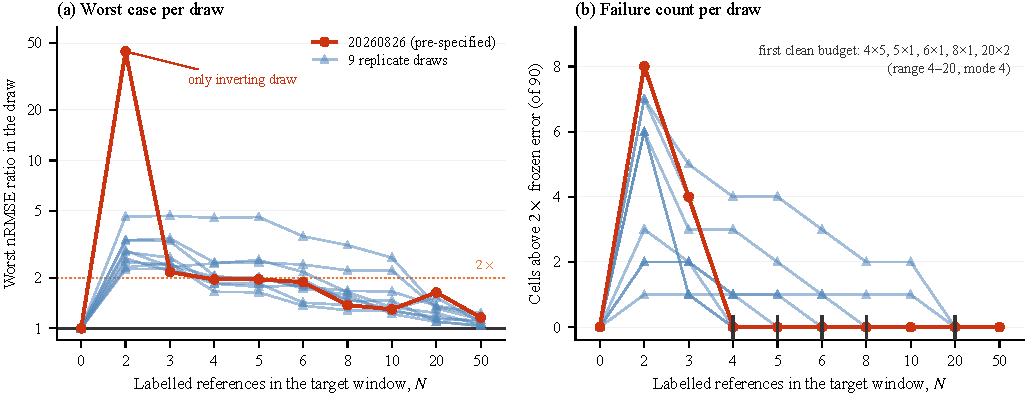
\includegraphics[width=\textwidth]{figure_05_draw_sensitivity.pdf}
\caption{The same protocol under 10 independent reference-panel draws, each redrawing every panel and reseeding the model random states; the pre-specified draw is highlighted. (a) Worst nRMSE ratio observed in each draw, logarithmic scale. Inversion and inflation beyond fivefold occur at two references and at no other budget in any draw, and only the pre-specified draw realises them; above two references the worst outcome anywhere is 4.7-fold. (b) Number of cells above twice frozen error, with a tick marking each draw's first clean budget. Those budgets are 4, 6, 4, 20, 20, 4, 4, 5, 8, 4, so the apparently clean threshold of the pre-specified draw is a property of that panel realisation and not of the method. Every draw uses the same range-spanning design, so the spread is not a consequence of poor transfer-sample selection.}
\label{fig:5}
\end{figure}


\clearpage

%% ---- Main tables ----

\begin{table}[htbp]
\centering
\caption{\textbf{Corpus and evaluation design.} Source windows 1--3 (2004-03-10 to 2004-06-08) fit each model; target windows 4--13 are evaluated one at a time. Within a target window the held-out test set is frozen before any reference is selected. Distinct target values are co-located reference-analyser readings, not nominal levels. Held-out rows are counted at the five-reference budget; they vary by at most the reference count across budgets.}
\label{tab:table1}
\small
\begin{adjustbox}{max width=\textwidth}
\begin{tabular}{llrrp{0.11\textwidth}p{0.13\textwidth}p{0.11\textwidth}}
\toprule
Analyte & Unit & Source rows & Windows & Rows/window & Distinct ref.\ values & Held-out rows \\
\midrule
CO & mg m$^{-3}$ & 1670 & 10 & 449--696 & 40--82 & 134--209 \\
NO2 & \si{\micro\gram\per\cubic\metre} & 1684 & 10 & 362--710 & 106--210 & 107--195 \\
NOx & ppb & 1684 & 10 & 363--710 & 148--478 & 105--198 \\
\bottomrule
\end{tabular}
\end{adjustbox}
\end{table}

\begin{sidewaystable}[htbp]
\centering
\caption{\textbf{Held-out error against reference budget, all four update strategies.} Mean over 90 decision cells per budget; \texttt{ratio} is the per-cell lightweight-to-frozen nRMSE ratio, so its mean is not the ratio of the displayed means. Cells > 2$\times$ counts cells whose held-out nRMSE exceeds twice that of the frozen model, and is the failure statistic used throughout. Inverted counts cells whose held-out calibration slope is negative. Cells are not independent replicates: they share source fits and target windows.}
\label{tab:table2}
\footnotesize
\setlength{\tabcolsep}{3pt}
\begin{adjustbox}{max width=\textheight}
\begin{tabular}{rrrrrrrrrr}
\toprule
N & Frozen & Lightweight & Target-only & Full retrain & Mean ratio & Median ratio & Cells $>2\times$ & Inverted & Improved \\
\midrule
0 & 0.18414 & 0.18414 & 0.18414 & 0.18414 & 1.000 & 1.000 & 0 & 0 & 0/90 \\
2 & 0.18414 & 0.29585 & 0.45609 & \textbf{0.17326} & 2.005 & 1.009 & 8 & 3 & 44/90 \\
3 & 0.18414 & \textbf{0.15913} & 0.20231 & 0.17215 & 1.035 & 0.992 & 4 & 0 & 45/90 \\
4 & 0.18414 & \textbf{0.13608} & 0.17755 & 0.16756 & 0.906 & 0.899 & 0 & 0 & 55/90 \\
5 & 0.18414 & \textbf{0.12930} & 0.15960 & 0.16599 & 0.877 & 0.857 & 0 & 0 & 59/90 \\
6 & 0.18414 & \textbf{0.12218} & 0.14546 & 0.15999 & 0.841 & 0.858 & 0 & 0 & 61/90 \\
8 & 0.18414 & \textbf{0.11446} & 0.13161 & 0.15635 & 0.793 & 0.837 & 0 & 0 & 62/90 \\
10 & 0.18414 & \textbf{0.11223} & 0.12450 & 0.15325 & 0.779 & 0.826 & 0 & 0 & 63/90 \\
20 & 0.18414 & \textbf{0.10857} & 0.11431 & 0.14006 & 0.757 & 0.834 & 0 & 0 & 70/90 \\
50 & 0.18414 & 0.10563 & \textbf{0.10265} & 0.12257 & 0.729 & 0.816 & 0 & 0 & 83/90 \\
\bottomrule
\end{tabular}
\end{adjustbox}
\end{sidewaystable}

\begin{sidewaystable}[htbp]
\centering
\caption{\textbf{Every cell above twice frozen error, with mechanism.} These are all 12 such cells in the corpus; none occur at any budget above N = 3. Held-out calibration slope is the slope of reference values regressed on predictions over the test set, where 1 is ideal. Inversion means that slope is negative, so the recalibrated model orders concentrations backwards. Slope error means the correction had the right sign but the wrong magnitude.}
\label{tab:table3}
\footnotesize
\setlength{\tabcolsep}{3pt}
\begin{adjustbox}{max width=\textheight}
\begin{tabular}{rlrlrrrrrl}
\toprule
N & Analyte & Window & Model & Frozen nRMSE & Lightweight nRMSE & Ratio & Held-out slope & $D_{\mathrm{ref}}$ & Mechanism \\
\midrule
2 & NO2 & 6 & PLS & 0.146 & 6.485 & 44.5$\times$ & $-$0.050 & 5.15 & Inversion \\
2 & NO2 & 6 & Random forest & 0.129 & 3.070 & 23.8$\times$ & $-$0.102 & 5.66 & Inversion \\
2 & NO2 & 6 & XGBoost & 0.138 & 2.732 & 19.8$\times$ & $-$0.120 & 5.94 & Inversion \\
2 & NO2 & 9 & PLS & 0.133 & 0.310 & 2.3$\times$ & 0.679 & 1.49 & Slope error \\
2 & NOx & 5 & PLS & 0.100 & 0.231 & 2.3$\times$ & 0.632 & 2.86 & Slope error \\
2 & NOx & 4 & Random forest & 0.090 & 0.200 & 2.2$\times$ & 0.658 & 2.19 & Slope error \\
2 & NOx & 4 & XGBoost & 0.090 & 0.190 & 2.1$\times$ & 0.683 & 1.97 & Slope error \\
2 & CO & 13 & XGBoost & 0.087 & 0.181 & 2.1$\times$ & 0.682 & 3.01 & Slope error \\
3 & NOx & 4 & Random forest & 0.090 & 0.195 & 2.2$\times$ & 0.626 & 1.67 & Slope error \\
3 & NOx & 5 & PLS & 0.100 & 0.209 & 2.1$\times$ & 0.605 & 2.21 & Slope error \\
3 & CO & 13 & XGBoost & 0.087 & 0.178 & 2.1$\times$ & 0.667 & 2.27 & Slope error \\
3 & NOx & 4 & XGBoost & 0.090 & 0.185 & 2.0$\times$ & 0.651 & 1.47 & Slope error \\
\bottomrule
\end{tabular}
\end{adjustbox}
\end{sidewaystable}

\begin{table}[htbp]
\centering
\caption{\textbf{Pre-specified hypothesis outcomes.} Thresholds were selected on rule-fitting windows 4--9 and applied unchanged to held-out windows 10--13. The rule-fitting windows overlap the span that generated the diagnostic hypothesis and are in-sample for hypothesis generation; windows 10--13 cover 121 days not used in any earlier analysis. The H2 means are over the 36 held-out cells at $N=20$ and are therefore not comparable with the 90-cell all-window means in Table 2.}
\label{tab:table4}
\small
\begin{adjustbox}{max width=\textwidth}
\begin{tabular}{p{0.13\textwidth}p{0.24\textwidth}p{0.20\textwidth}p{0.22\textwidth}p{0.11\textwidth}}
\toprule
Hypothesis & Pre-specified test & Rule-fitting windows 4--9 & Held-out windows 10--13 & Verdict \\
\midrule
H1 diagnostic validity & Spearman $\rho(D_{\mathrm{ref}}(5), \Delta\mathrm{nRMSE}) > 0$, $p < 0.05$ & $\rho=0.348$, $p=0.01$ ($n=54$) & $\rho=0.814$, $p=1.6\times 10^{-9}$ ($n=36$) & \textbf{SUPPORTED} \\
H2 rule utility & Rule beats always-frozen \emph{and} always-recalibrate on mean held-out nRMSE & selected $\tau=0.10$, $N=20$ & frozen 0.2412, recalibrate 0.1176, rule 0.1176 & \textbf{SUPPORTED}, practically null \\
H3 decision cheaper than fit & Action agreement reaches 100 \% at smaller $N$ than the fitting plateau & --- & decision-stable at $N=10$, fit plateau at $N=20$ & \textbf{SUPPORTED} \\
\bottomrule
\end{tabular}
\end{adjustbox}
\end{table}

\begin{sidewaystable}[htbp]
\centering
\caption{\textbf{The failure threshold does not replicate across reference-panel draws.} Each draw redraws every panel and reseeds the model random states, so each is an independent realisation of the same range-spanning design. Counts are cells above twice frozen error, of 90 per budget. The final column is the smallest budget from which that draw and all larger budgets are clean. Reported post-hoc; no threshold, hypothesis, or verdict of the frozen protocol is changed.}
\label{tab:table5}
\footnotesize
\setlength{\tabcolsep}{3pt}
\begin{adjustbox}{max width=\textheight}
\begin{tabular}{lrrrrrrrrrr}
\toprule
Draw & N=2 & N=3 & N=4 & N=5 & N=6 & N=8 & N=10 & N=20 & N=50 & First clean $N$ \\
\midrule
\textbf{20260826} (pre-specified) & 8 & 4 & 0 & 0 & 0 & 0 & 0 & 0 & 0 & \textbf{4} \\
11 & 2 & 2 & 1 & 1 & 0 & 0 & 0 & 0 & 0 & \textbf{6} \\
22 & 1 & 1 & 0 & 0 & 0 & 0 & 0 & 0 & 0 & \textbf{4} \\
33 & 6 & 3 & 3 & 2 & 1 & 1 & 1 & 0 & 0 & \textbf{20} \\
44 & 7 & 5 & 4 & 4 & 3 & 2 & 2 & 0 & 0 & \textbf{20} \\
55 & 3 & 2 & 0 & 0 & 0 & 0 & 0 & 0 & 0 & \textbf{4} \\
66 & 7 & 4 & 0 & 0 & 0 & 0 & 0 & 0 & 0 & \textbf{4} \\
77 & 2 & 2 & 1 & 0 & 0 & 0 & 0 & 0 & 0 & \textbf{5} \\
88 & 6 & 1 & 1 & 1 & 1 & 0 & 0 & 0 & 0 & \textbf{8} \\
99 & 6 & 1 & 0 & 0 & 0 & 0 & 0 & 0 & 0 & \textbf{4} \\
\bottomrule
\end{tabular}
\end{adjustbox}
\end{sidewaystable}

\begin{sidewaystable}[htbp]
\centering
\caption{\textbf{Draw-invariant results, pooled over 10 panel draws (900 cells per budget).} The worst observed ratio requires no threshold and is the quantity a prohibition bounds. Slope inversion and inflation beyond fivefold occur at N = 2 and at no other budget in any draw, which is what the exact-determination argument of Section 2.1 predicts. Counts above 2$\times$ decay gradually and reach zero only at N = 20, so no small panel is reliably safe.}
\label{tab:table6}
\footnotesize
\setlength{\tabcolsep}{3pt}
\begin{adjustbox}{max width=\textheight}
\begin{tabular}{rrrrrrrrrrr}
\toprule
N & Cells & Worst nRMSE & Worst MAE & Inverted & >5$\times$ & >3$\times$ & >2$\times$ & $>2\times$ MAE & Mean ratio & Median ratio \\
\midrule
0 & 900 & 1.00 & 1.00 & 0 & 0 & 0 & 0 & 0 & 1.000 & 1.000 \\
2 & 900 & 44.53 & 50.99 & 3 & 3 & 7 & 48 & 67 & 1.169 & 1.017 \\
3 & 900 & 4.68 & 4.41 & 0 & 0 & 4 & 25 & 34 & 1.012 & 0.988 \\
4 & 900 & 4.54 & 4.27 & 0 & 0 & 2 & 10 & 11 & 0.908 & 0.930 \\
5 & 900 & 4.60 & 4.27 & 0 & 0 & 2 & 8 & 10 & 0.880 & 0.905 \\
6 & 900 & 3.53 & 3.52 & 0 & 0 & 2 & 5 & 6 & 0.841 & 0.880 \\
8 & 900 & 3.13 & 2.99 & 0 & 0 & 2 & 3 & 3 & 0.799 & 0.849 \\
10 & 900 & 2.63 & 2.36 & 0 & 0 & 0 & 3 & 3 & 0.779 & 0.831 \\
20 & 900 & 1.64 & 1.70 & 0 & 0 & 0 & 0 & 0 & 0.748 & 0.810 \\
50 & 900 & 1.23 & 1.22 & 0 & 0 & 0 & 0 & 0 & 0.727 & 0.795 \\
\bottomrule
\end{tabular}
\end{adjustbox}
\end{sidewaystable}


\clearpage

%% ---- Supplementary tables ----

\begin{sidewaystable}[htbp]
\centering
\caption{\textbf{Per-analyte and per-model detail at the floor and at the primary budget.} Medians over the ten target windows. $\Delta$nRMSE is the median of the per-window frozen-minus-lightweight differences and need not equal the difference of the displayed medians. Positive $\Delta$nRMSE favours recalibration.}
\label{tab:tables1}
\footnotesize
\setlength{\tabcolsep}{3pt}
\begin{adjustbox}{max width=\textheight}
\begin{tabular}{llrrrrrrr}
\toprule
Analyte & Model & Frozen nRMSE & N=4 lightweight & N=4 $\Delta$nRMSE & N=4 improved & N=5 lightweight & N=5 $\Delta$nRMSE & N=5 improved \\
\midrule
CO & PLS & 0.102 & 0.093 & +0.0001 & 5/10 & 0.094 & +0.0015 & 6/10 \\
CO & Random forest & 0.076 & 0.083 & $-$0.0028 & 4/10 & 0.084 & $-$0.0023 & 5/10 \\
CO & XGBoost & 0.078 & 0.090 & $-$0.0065 & 3/10 & 0.089 & $-$0.0037 & 4/10 \\
NO2 & PLS & 0.138 & 0.124 & +0.0142 & 6/10 & 0.126 & +0.0134 & 6/10 \\
NO2 & Random forest & 0.179 & 0.146 & +0.0122 & 8/10 & 0.144 & +0.0336 & 9/10 \\
NO2 & XGBoost & 0.182 & 0.145 & +0.0227 & 8/10 & 0.135 & +0.0389 & 8/10 \\
NOx & PLS & 0.353 & 0.148 & +0.1599 & 7/10 & 0.153 & +0.1873 & 7/10 \\
NOx & Random forest & 0.322 & 0.148 & +0.1619 & 7/10 & 0.142 & +0.1695 & 7/10 \\
NOx & XGBoost & 0.331 & 0.160 & +0.1655 & 7/10 & 0.144 & +0.1733 & 7/10 \\
\bottomrule
\end{tabular}
\end{adjustbox}
\end{sidewaystable}

\begin{table}[htbp]
\centering
\caption{\textbf{Panel geometry of the inversion cells.} The reference panel is ordered to span the target range, so at N = 2 the two references are the extreme low and high strata of the window. For a two-point panel the least-squares calibrator coefficient is exactly the ratio of the true gap to the predicted gap. In NO2 window 6 all three frozen models compress a 91 \si{\micro\gram\per\cubic\metre} interval into 4--12 \si{\micro\gram\per\cubic\metre} \textbf{of the wrong sign}, so the coefficient is large and negative and every prediction is inverted. The calibrator coefficient below is the multiplier applied to the frozen output; it is a different quantity from the held-out calibration slope in Table 3.}
\label{tab:tables2}
\small
\begin{adjustbox}{max width=\textwidth}
\begin{tabular}{lp{0.13\textwidth}p{0.17\textwidth}rrrr}
\toprule
Model & Ref.\ values & Frozen pred. & True gap & Predicted gap & Calib.\ coef. & Held-out ratio \\
\midrule
PLS & 27, 118 & 116.603, 112.334 & +91.0 & $-$4.27 & $-$21.32 & 44.5$\times$ \\
Random forest & 27, 118 & 117.320, 107.660 & +91.0 & $-$9.66 & $-$9.42 & 23.8$\times$ \\
XGBoost & 27, 118 & 122.641, 110.944 & +91.0 & $-$11.70 & $-$7.78 & 19.8$\times$ \\
\bottomrule
\end{tabular}
\end{adjustbox}
\end{table}

\begin{table}[htbp]
\centering
\caption{\textbf{Why N = 2 cannot be checked from its own panel.} A two-parameter calibrator fitted on two points reproduces both exactly, so the panel residual is identically zero and no panel-internal evidence of failure can exist. From N = 3 the panel can contradict the fitted line. Rank agreement is the fraction of reference pairs the frozen model orders correctly. This table is post-hoc: it was constructed after the failures were observed and is reported as mechanism, not as a decision rule.}
\label{tab:tables3}
\small
\begin{adjustbox}{max width=\textwidth}
\begin{tabular}{lrlp{0.15\textwidth}rrrr}
\toprule
N & Res.\ d.f. & Med.\ residual & Min rank agr. & Cells > 2$\times$ \\
\midrule
2 & 0 & 0.000 & 0.000 & 8 \\
3 & 1 & 4.547 & 0.333 & 4 \\
4 & 2 & 11.346 & 0.500 & 0 \\
5 & 3 & 14.202 & 0.500 & 0 \\
6 & 4 & 15.886 & 0.600 & 0 \\
8 & 6 & 18.014 & 0.679 & 0 \\
Analyte & Window & Model & Reference values & Rank agreement \\
--- & ---: & --- & --- & ---: \\
CO & 13 & XGBoost & 0.5, 0.7, 4.9 & 1.000 \\
NOx & 4 & Random forest & 30, 40, 261 & 1.000 \\
NOx & 4 & XGBoost & 30, 40, 261 & 1.000 \\
NOx & 5 & PLS & 14, 47, 275 & 1.000 \\
\bottomrule
\end{tabular}
\end{adjustbox}
\end{table}

\begin{table}[htbp]
\centering
\caption{\textbf{Target distribution of the NO2 windows}, as observed before the common-support restriction and before the held-out split. Window 6, which carries every inversion cell, has the fewest rows, the fewest distinct reference values, the lowest mean concentration, and the strongest right skew of the ten windows. Its range is not the narrowest: window 8 spans 165 against window 6's 166.}
\label{tab:tables4}
\footnotesize
\begin{adjustbox}{max width=\textwidth}
\begin{tabular}{rrrrrrrr}
\toprule
Window & Rows & Distinct & Min & Max & Range & Mean & Skew \\
\midrule
4 & 652 & 169 & 16 & 233 & 217 & 103.6 & 0.34 \\
5 & 655 & 160 & 5 & 206 & 201 & 98.6 & 0.25 \\
\textbf{6} & 362 & 106 & 5 & 171 & 166 & 66.0 & 0.60 \\
7 & 428 & 166 & 2 & 225 & 223 & 108.5 & 0.16 \\
8 & 479 & 132 & 29 & 194 & 165 & 89.5 & 0.56 \\
9 & 658 & 208 & 13 & 288 & 275 & 126.0 & 0.34 \\
10 & 478 & 158 & 27 & 269 & 242 & 123.0 & 0.34 \\
11 & 672 & 200 & 17 & 333 & 316 & 137.9 & 0.27 \\
12 & 615 & 210 & 25 & 310 & 285 & 154.2 & 0.10 \\
13 & 710 & 191 & 29 & 248 & 219 & 132.3 & 0.23 \\
\bottomrule
\end{tabular}
\end{adjustbox}
\end{table}

\begin{table}[htbp]
\centering
\caption{\textbf{Threshold and endpoint sensitivity within the pre-specified draw.} The budget at which failures cease depends on the tolerance and on the error metric, independently of the panel draw. Neither choice is canonical, so a laboratory with a defined tolerance should read the relevant column rather than adopt the twofold nRMSE convention used in the main text.}
\label{tab:tables5}
\small
\begin{adjustbox}{max width=\textwidth}
\begin{tabular}{rrrrrr}
\toprule
N & $>1.5\times$ & $>2\times$ & $>3\times$ & $>5\times$ & $>2\times$ MAE \\
\midrule
0 & 0 & 0 & 0 & 0 & 0 \\
2 & 18 & 8 & 3 & 3 & 9 \\
3 & 14 & 4 & 0 & 0 & 5 \\
4 & 6 & 0 & 0 & 0 & 1 \\
5 & 5 & 0 & 0 & 0 & 1 \\
6 & 3 & 0 & 0 & 0 & 1 \\
8 & 0 & 0 & 0 & 0 & 0 \\
10 & 0 & 0 & 0 & 0 & 0 \\
20 & 2 & 0 & 0 & 0 & 0 \\
50 & 0 & 0 & 0 & 0 & 0 \\
Criterion & First clean N &  &  &  &  \\
--- & ---: &  &  &  &  \\
nRMSE ratio > 1.5 & 50 &  &  &  &  \\
nRMSE ratio > 2.0 & 4 &  &  &  &  \\
nRMSE ratio > 3.0 & 3 &  &  &  &  \\
nRMSE ratio > 5.0 & 3 &  &  &  &  \\
MAE ratio > 2.0 & 8 &  &  &  &  \\
\bottomrule
\end{tabular}
\end{adjustbox}
\end{table}


\clearpage

\begin{thebibliography}{99}
\bibitem{ref1} A. Rudnitskaya, Calibration update and drift correction for electronic noses and tongues, Front. Chem. 6 (2018) 433. \newblock \href{https://doi.org/10.3389/fchem.2018.00433}{10.3389/fchem.2018.00433}
\bibitem{ref2} H. Chai, Z. Zheng, K. Liu, J. Xu, K. Wu, Y. Luo, H. Liao, M. Debliquy, C. Zhang, Stability of metal oxide semiconductor gas sensors: A review, IEEE Sens. J. 22 (2022) 5470--5481. \newblock \href{https://doi.org/10.1109/JSEN.2022.3148264}{10.1109/JSEN.2022.3148264}
\bibitem{ref3} R. Piedrahita, Y. Xiang, N. Masson, J. Ortega, A. Collier, Y. Jiang, K. Li, R.P. Dick, Q. Lv, M. Hannigan, L. Shang, The next generation of low-cost personal air quality sensors for quantitative exposure monitoring, Atmos. Meas. Tech. 7 (2014) 3325--3336. \newblock \href{https://doi.org/10.5194/amt-7-3325-2014}{10.5194/amt-7-3325-2014}
\bibitem{ref4} Y. Wang, D.J. Veltkamp, B.R. Kowalski, Multivariate instrument standardization, Anal. Chem. 63 (1991) 2750--2756. \newblock \href{https://doi.org/10.1021/ac00023a016}{10.1021/ac00023a016}
\bibitem{ref5} T. Fearn, Standardisation and calibration transfer for near infrared instruments: A review, J. Near Infrared Spectrosc. 9 (2001) 229--244. \newblock \href{https://doi.org/10.1255/jnirs.309}{10.1255/jnirs.309}
\bibitem{ref6} E. Bouveresse, D.L. Massart, Improvement of the piecewise direct standardisation procedure for the transfer of NIR spectra for multivariate calibration, Chemom. Intell. Lab. Syst. 32 (1996) 201--213. \newblock \href{https://doi.org/10.1016/0169-7439(95)00074-7}{10.1016/0169-7439(95)00074-7}
\bibitem{ref7} S.D. Brown, Transfer of multivariate calibration models, in: Comprehensive Chemometrics, Elsevier, 2009, pp. 345--378. \newblock \href{https://doi.org/10.1016/B978-044452701-1.00077-6}{10.1016/B978-044452701-1.00077-6}
\bibitem{ref8} A. Vergara, S. Vembu, T. Ayhan, M.A. Ryan, M.L. Homer, R. Huerta, Chemical gas sensor drift compensation using classifier ensembles, Sens. Actuators B Chem. 166--167 (2012) 320--329. \newblock \href{https://doi.org/10.1016/j.snb.2012.01.074}{10.1016/j.snb.2012.01.074}
\bibitem{ref9} H. Liu, Z. Tang, Metal oxide gas sensor drift compensation using a dynamic classifier ensemble based on fitting, Sensors 13 (2013) 9160--9173. \newblock \href{https://doi.org/10.3390/s130709160}{10.3390/s130709160}
\bibitem{ref10} S. Lu, J. Guo, S. Liu, B. Yang, M. Liu, L. Yin, W. Zheng, An improved algorithm of drift compensation for olfactory sensors, Appl. Sci. 12 (2022) 9529. \newblock \href{https://doi.org/10.3390/app12199529}{10.3390/app12199529}
\bibitem{ref11} Y. Yao, B. Chen, C. Liu, C. Qu, Investigation on the combined model of sensor drift compensation and open-set gas recognition based on electronic nose datasets, Chemom. Intell. Lab. Syst. 242 (2023) 105003. \newblock \href{https://doi.org/10.1016/j.chemolab.2023.105003}{10.1016/j.chemolab.2023.105003}
\bibitem{ref12} M. Padilla, A. Perera, I. Montoliu, A. Chaudry, K. Persaud, S. Marco, Drift compensation of gas sensor array data by orthogonal signal correction, Chemom. Intell. Lab. Syst. 100 (2010) 28--35. \newblock \href{https://doi.org/10.1016/j.chemolab.2009.10.002}{10.1016/j.chemolab.2009.10.002}
\bibitem{ref13} A. Ziyatdinov, S. Marco, A. Chaudry, K. Persaud, P. Caminal, A. Perera, Drift compensation of gas sensor array data by common principal component analysis, Sens. Actuators B Chem. 146 (2010) 460--465. \newblock \href{https://doi.org/10.1016/j.snb.2009.11.034}{10.1016/j.snb.2009.11.034}
\bibitem{ref14} H. Liu, R. Chu, Z. Tang, Metal oxide gas sensor drift compensation using a two-dimensional classifier ensemble, Sensors 15 (2015) 10180--10193. \newblock \href{https://doi.org/10.3390/s150510180}{10.3390/s150510180}
\bibitem{ref15} K. Yan, D. Zhang, Calibration transfer and drift compensation of e-noses via coupled task learning, Sens. Actuators B Chem. 225 (2016) 288--297. \newblock \href{https://doi.org/10.1016/j.snb.2015.11.058}{10.1016/j.snb.2015.11.058}
\bibitem{ref16} Z. Jiang, P. Xu, Y. Du, F. Yuan, K. Song, Balanced distribution adaptation for metal oxide semiconductor gas sensor array drift compensation, Sensors 21 (2021) 3403. \newblock \href{https://doi.org/10.3390/s21103403}{10.3390/s21103403}
\bibitem{ref17} S. De Vito, G. Fattoruso, M. Pardo, F. Tortorella, G. Di Francia, Semi-supervised learning techniques in artificial olfaction: A novel approach to classification problems and drift counteraction, IEEE Sens. J. 12 (2012) 3215--3224. \newblock \href{https://doi.org/10.1109/JSEN.2012.2192425}{10.1109/JSEN.2012.2192425}
\bibitem{ref18} X. Dong, S. Han, A. Wang, K. Shang, Online inertial machine learning for sensor array long-term drift compensation, Chemosensors 9 (2021) 353. \newblock \href{https://doi.org/10.3390/chemosensors9120353}{10.3390/chemosensors9120353}
\bibitem{ref19} J. Lin, X. Zhan, Sensor-drift compensation in electronic-nose-based gas recognition using knowledge distillation, Informatics 13 (2026) 15. \newblock \href{https://doi.org/10.3390/informatics13010015}{10.3390/informatics13010015}
\bibitem{ref20} P. Maho, C. Herrier, T. Livache, P. Comon, S. Barthelm\'e, A calibrant-free drift compensation method for gas sensor arrays, Chemom. Intell. Lab. Syst. 225 (2022) 104549. \newblock \href{https://doi.org/10.1016/j.chemolab.2022.104549}{10.1016/j.chemolab.2022.104549}
\bibitem{ref21} S. De Vito, G. Di Francia, E. Esposito, S. Ferlito, F. Formisano, E. Massera, Adaptive machine learning strategies for network calibration of IoT smart air quality monitoring devices, Pattern Recognit. Lett. 136 (2020) 264--271. \newblock \href{https://doi.org/10.1016/j.patrec.2020.04.032}{10.1016/j.patrec.2020.04.032}
\bibitem{ref22} S. De Vito, E. Massera, M. Piga, L. Martinotto, G. Di Francia, On field calibration of an electronic nose for benzene estimation in an urban pollution monitoring scenario, Sens. Actuators B Chem. 129 (2008) 750--757. \newblock \href{https://doi.org/10.1016/j.snb.2007.09.060}{10.1016/j.snb.2007.09.060}
\bibitem{ref23} S. De Vito, M. Piga, L. Martinotto, G. Di Francia, CO, NO2 and NOx urban pollution monitoring with on-field calibrated electronic nose by automatic Bayesian regularization, Sens. Actuators B Chem. 143 (2009) 182--191. \newblock \href{https://doi.org/10.1016/j.snb.2009.08.041}{10.1016/j.snb.2009.08.041}
\bibitem{ref24} S. De Vito, Air Quality, UCI Machine Learning Repository, 2008. \newblock \href{https://doi.org/10.24432/C59K5F}{10.24432/C59K5F}
\bibitem{ref25} J. W\"orner, J. Eimler, M. Pein-Hackelbusch, Long-term drift behavior in metal oxide gas sensor arrays: A one-year dataset from an electronic nose, Sci. Data 12 (2025). \newblock \href{https://doi.org/10.1038/s41597-025-05993-8}{10.1038/s41597-025-05993-8}
\bibitem{ref26} C. Bergmeir, R.J. Hyndman, B. Koo, A note on the validity of cross-validation for evaluating autoregressive time series prediction, Comput. Stat. Data Anal. 120 (2018) 70--83. \newblock \href{https://doi.org/10.1016/j.csda.2017.11.003}{10.1016/j.csda.2017.11.003}
\bibitem{ref27} V. Cerqueira, L. Torgo, I. Mozeti\v{c}, Evaluating time series forecasting models: An empirical study on performance estimation methods, Mach. Learn. 109 (2020) 1997--2028. \newblock \href{https://doi.org/10.1007/s10994-020-05910-7}{10.1007/s10994-020-05910-7}
\bibitem{ref28} D.R. Roberts, V. Bahn, S. Ciuti, et al., Cross-validation strategies for data with temporal, spatial, hierarchical, or phylogenetic structure, Ecography 40 (2017) 913--929. \newblock \href{https://doi.org/10.1111/ecog.02881}{10.1111/ecog.02881}
\bibitem{ref29} S. Kaufman, S. Rosset, C. Perlich, O. Stitelman, Leakage in data mining, ACM Trans. Knowl. Discov. Data 6 (2012) 1--21. \newblock \href{https://doi.org/10.1145/2382577.2382579}{10.1145/2382577.2382579}
\bibitem{ref30} N. Dennler, S. Rastogi, J. Fonollosa, A. van Schaik, M. Schmuker, Drift in a popular metal oxide sensor dataset reveals limitations for gas classification benchmarks, Sens. Actuators B Chem. 361 (2022) 131668. \newblock \href{https://doi.org/10.1016/j.snb.2022.131668}{10.1016/j.snb.2022.131668}
\end{thebibliography}

\end{document}
